% !Mode:: "TeX:UTF-8"
\documentclass[10pt,punct]{ctexbeamer}
%\usepackage[utf8]{inputenc}
% fontset=mac
\usefonttheme[onlymath]{serif}


\usepackage{amsmath,amssymb,amsthm}             % AMS Math
%\usepackage[T1]{fontenc}
\usepackage{graphicx}
\usepackage{epstopdf}
\usepackage{tikz}
\linespread{1.3}

\usepackage{mathrsfs}  %花写字母
\usepackage{colortbl}  %彩色表格需要加载的宏包

%%%=== theme ===%%%
% \usetheme{Warsaw}
%\usetheme{Copenhagen}
%\usetheme{Singapore}
\usetheme{Madrid}
%\usefonttheme{professionalfonts}
%\usefonttheme{serif}
% \usefonttheme{structureitalicserif}
%%\useinnertheme{rounded}
%%\useinnertheme{inmargin}
\useinnertheme{circles}
%\useoutertheme{miniframes}
\setbeamertemplate{navigation symbols}{}
\setbeamertemplate{footline}[frame number]

\titlegraphic{
\includegraphics[width=2cm]{../tjnu.jpg}}

%\usepackage[fontset=mac]{ctex}
%\usepackage{ctex}
% \usepackage{CJK,CJKnumb,CJKulem}
%\usepackage{minitoc}


\setbeamertemplate{theorems}[numbered]
\newtheorem{thm}{定理}
\newtheorem{lem}{引理}
\newtheorem{ex}{例}
\newtheorem*{theo}{定理}
\newtheorem*{conj}{猜想}
\newtheorem*{defi}{定义}
\newtheorem*{coro}{推论}
\newtheorem*{rem}{注}
\newtheorem*{prop}{性质}
\newtheorem{pr1}{性质}
\newtheorem{pr2}{性质}
\newtheorem{pr3}{性质}
\newtheorem*{qst}{问题}

\def\qed{\nopagebreak\hfill{\rule{4pt}{7pt}}\medbreak}
\def\pf{{\bf 证明~~ }}
\def\sol{{\bf 解~~ }}



\def\R{\mathbb{R}}
\def\Rn{\mathbb{R}^n}
\def\A{\mathscr{A}}
\def\B{\mathscr{B}}
\def\D{\mathscr{D}}
\def\E{\mathscr{E}}
\def\O{\mathscr{O}}
\def\e{\mathrm{e}}
\def\i{\, \mathrm{i}}

\def\rank{\operatorname{rank}}
\def\dim{\operatorname{dim}}
\def\0{\mathbf{0}}
\def\a{\alpha}
\def\b{\beta}
\def\r{\gamma}

\usepackage{graphicx}
\usepackage{color}
\definecolor{linkcol}{rgb}{0,0,0.4}
\definecolor{citecol}{rgb}{0.5,0,0}

\definecolor{blue}{rgb}{0,0.08,1}
\newcommand{\blue}{\textcolor{blue}}


%  \DeclareGraphicsExtensions{.eps}
%   \usepackage[a4paper,pagebackref,hyperindex=true,pdfnewwindow=true]{hyperref}


\begin{document}



\title[]{行列式的几何解释}
\author[]{{\large 张彪} }
\institute[]{{\normalsize
		天津师范大学\\[4pt]
        数学科学学院\\[10pt]
		zhang@tjnu.edu.cn}}

\date{}


%
%\AtBeginSection[]
%{
%\begin{frame}
%	\frametitle{提纲}
%	\tableofcontents[currentsection]
%\end{frame}
%}
%


\begin{frame}
\maketitle
\end{frame}

%\begin{frame}
%\frametitle{\textcolor{orange}{提纲}}
%\tableofcontents
%\end{frame}
%



\begin{frame}{平行四边形的面积与二阶行列式}

    \begin{columns}[c]
        \column{8cm}

        对任意 $\overrightarrow{O A}=\left(\begin{array}{l}a_1 \\ a_2\end{array}\right), \overrightarrow{O B}=\left(\begin{array}{l}b_1 \\ b_2\end{array}\right)$

        将 $O B$ 绕 $O$ 沿顺时针方向旋转直角得到有向线 段 $O B^{\, \prime}$. 则 $\overrightarrow{O B^{\, \prime}}=\left(\begin{array}{r}b_2 \\ -b_1\end{array}\right)$.


        %则 $\overrightarrow{O B^{\, \prime}}=\left( b_2, -b_1 \right)$.

        考虑$\Delta=a_1 b_2-a_2 b_1$, 它就是 $\overrightarrow{O A} \cdot \overrightarrow{O B^{\, \prime}}$.

        由于 $\left|O B^{\, \prime}\right|=|O B|, \angle B O B^{\, \prime}=$ $-\frac{\pi}{2}$, 于是
        %        \pause
        $$
        \begin{aligned}
            \Delta=\overrightarrow{O A} \cdot \overrightarrow{O B^{\, \prime}}
            & = |O A|\left|O B^{\, \prime}\right| \cos \angle A O B^{\, \prime}\\
            & = |O A||O B| \cos \left(\angle A O B-\frac{\pi}{2}\right) \\
            & = |O A||O B| \sin \angle A O B
        \end{aligned}
        $$


        \column{4.5cm}
        \begin{figure}[p]
            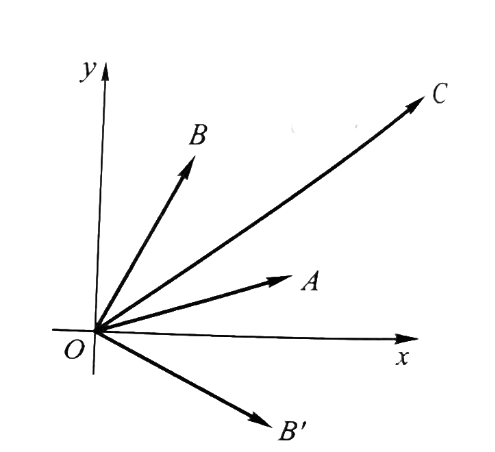
\includegraphics[scale=0.2]{det-2.jpeg}
            %    \caption{}
        \end{figure}

        \pause
        \begin{itemize}
            \item  $\triangle$ 的\alert{绝对值}就是以 $O A, O B$ 为一组邻边的平行四边形 $O A P B$ 的面积 $S_{O A P B}$
            \item   $\triangle$ 的\alert{符号}就是 $\sin \angle A O B$ 的符号
        \end{itemize}


    \end{columns}



\end{frame}

\begin{frame}


    对任意 $\overrightarrow{O A}=\left(\begin{array}{l}a_1 \\ a_2\end{array}\right), \overrightarrow{O B}=\left(\begin{array}{l}b_1 \\ b_2\end{array}\right)$, 定义 $$\operatorname{det}(\overrightarrow{O A}, \overrightarrow{O B})=|O A||O B| \sin \angle A O B$$

    也记作
    $$\operatorname{det}\left(\begin{array}{ll}a_1 & b_1 \\ a_2 & b_2\end{array}\right) \mbox{ 或  } \quad \left|\begin{array}{ll}a_1 & b_1 \\ a_2 & b_2\end{array}\right|$$


    称为\alert{二阶行列式}.

    将它理解为平行四边形 OAPB 的\alert{有向 面积},

    取值既可以为正实数, 也可以取负实数或零.
\end{frame}

\begin{frame}


    它具有如下基本性质:

    \begin{pr1}
        $\operatorname{det}\left(x_1 \boldsymbol{\alpha}_1+x_2 \boldsymbol{\alpha}_2, y_1 \boldsymbol{\beta}_1+y_2 \boldsymbol{\beta}_2\right)=\sum_{i, j=1}^2 x_i y_j \operatorname{det}\left(\boldsymbol{\alpha}_i, \boldsymbol{\beta}_j\right)$.
    \end{pr1}

    也就是说:可以将 $\operatorname{det}(\boldsymbol{\alpha}, \boldsymbol{\beta})$ 看作向量 $\boldsymbol{\alpha}$ 与 $\boldsymbol{\beta}$ 的某种乘积, 按乘法对于加 法的分配律和与数乘的结合律展开.


    \begin{pr1}
        $\operatorname{det}(\boldsymbol{\alpha}, \boldsymbol{\alpha})=0, \quad  \operatorname{det}(\boldsymbol{\alpha}, \boldsymbol{\beta})=-\operatorname{det}(\boldsymbol{\beta}, \boldsymbol{\alpha})$.
    \end{pr1}
    也就是说: 两条棱重合, 面积为 0 ; 两条棱互相交换位置, 有向面积变号 (因为夹角 $\langle\alpha, \beta\rangle$ 的正弦变号: $\sin \langle\boldsymbol{\alpha}, \boldsymbol{\beta}\rangle=-\sin \langle\boldsymbol{\beta}, \boldsymbol{\alpha}\rangle$ ).


    \begin{pr1}
        $\operatorname{det}\left(\boldsymbol{e}_1, \boldsymbol{e}_2\right)=1$,
        其中 $\boldsymbol{e}_1=\left(\begin{array}{l}1 \\ 0\end{array}\right), \boldsymbol{e}_2=\left(\begin{array}{l}0 \\ 1\end{array}\right)$ 分别是 $x$ 轴、 $y$ 轴正方向的单位向量.
    \end{pr1}


\end{frame}


\begin{frame}
    前面已经通过$\overrightarrow{O A} \cdot \overrightarrow{O B^{\, \prime}}$ 计算出
    $$\operatorname{det}(\overrightarrow{O A}, \overrightarrow{O B})=\left|\begin{array}{ll}a_1 & b_1 \\ a_2 & b_2\end{array}\right|=a_1 b_2-a_2 b_1.$$


    为了推广到任意 $n$ 阶行列式, 我们反过来利用上面的三条基本性质来求二阶行列式:
    $$\begin{aligned} \Delta &=\left|\begin{array}{cc}a_1 & b_1 \\ a_2 & b_2\end{array}\right|=\operatorname{det}\left(a_1 \boldsymbol{e}_1+a_2 \boldsymbol{e}_2, b_1 \boldsymbol{e}_1+b_2 \boldsymbol{e}_2\right) \\
        & = a_1 b_1 \operatorname{det}\left(\boldsymbol{e}_1, \boldsymbol{e}_1\right)
        +a_1 b_2 \operatorname{det}\left(\boldsymbol{e}_1, \boldsymbol{e}_2\right)\\
        & \qquad
        +a_2 b_1 \operatorname{det}\left(\boldsymbol{e}_2, \boldsymbol{e}_1\right)
        +a_2 b_2 \operatorname{det}\left(\boldsymbol{e}_2, \boldsymbol{e}_2\right) \\
        & = a_1 b_1 \times 0+a_1 b_2 \times 1+a_2 b_1 \times(-1)+a_2 b_2 \times 0 \\ &=a_1 b_2-a_2 b_1 \end{aligned}$$
    显然, 有向面积 $\operatorname{det}(\overrightarrow{O A}, \overrightarrow{O B})=0 \Leftrightarrow O A, O B$ 共线.


    反过来, $\overrightarrow{O A}, \overrightarrow{O B}$ 组成平面$\mathbb{R}^2$上的一组基 $\Leftrightarrow \operatorname{det}(\overrightarrow{O A}, \overrightarrow{O B}) \neq 0$.

\end{frame}


\begin{frame}{平行六面 体的体积与三阶行列式}

    与二阶行列式类似, 对于 3 维几何空间 $\mathbb{R}^3$ 中的任意 3 个向量 $\boldsymbol{\alpha}=\overrightarrow{O A}= \left(\begin{array}{l}a_1 \\ a_2 \\ a_3\end{array}\right), \,
    \boldsymbol{\beta} =\overrightarrow{O B}= \left(\begin{array}{l}b_1 \\ b_2 \\ b_3\end{array}\right), \,
    \boldsymbol{\gamma}=\overrightarrow{O C}= \left(\begin{array}{l}c_1 \\ c_2 \\ c_3\end{array}\right)$,

    它们的混合积
    \begin{align*}
        \boldsymbol{\alpha} \cdot(\boldsymbol{\beta} \times \boldsymbol{\gamma})
        & =a_1\left|\begin{array}{cc}b_2 & b_3 \\ c_2 & c_3\end{array}\right|-a_2\left|\begin{array}{cc}b_1 & b_3 \\ c_1 & c_3\end{array}\right|+a_3\left|\begin{array}{cc}b_1 & b_2 \\ c_1 & c_2\end{array}\right|\\
        & = \left|\begin{array}{lll}a_1 & b_1 & c_1 \\ a_2 & b_2 & c_2 \\ a_3 & b_3 & c_3\end{array}\right|
    \end{align*}
    就是以 $O A, O B, O C$ 为三条棱的平行六面 体的\alert{有向体积}, 我们将它记为 $$\operatorname{det}(\boldsymbol{\alpha}, \boldsymbol{\beta}, \boldsymbol{\gamma}),$$ 称为\alert{三阶行列式}.

\end{frame}

\begin{frame}
    它也具有 3 条 基本性质:

    \begin{pr2}
        可以看作 $\boldsymbol{\alpha}, \boldsymbol{\beta}, \boldsymbol{\gamma}$ 的某种乘积, 按照乘法对于加法的分配律及 与数乘的分配律展开:
        $$
        \operatorname{det}\left(\sum_i x_i \boldsymbol{\alpha}_i, \sum_j y_j \boldsymbol{\beta}_j, \sum_k z_k \boldsymbol{\gamma}_k\right)=\sum_{i, j, k} x_i y_j z_k \operatorname{det}\left(\boldsymbol{\alpha}_i, \boldsymbol{\beta}_j, \boldsymbol{\gamma}_k\right)
        $$
    \end{pr2}
    \begin{pr2}
        \begin{itemize}
            \item 如果三个向量 $\boldsymbol{\alpha}, \boldsymbol{\beta}, \boldsymbol{\gamma}$ 中有两个相等, 则平行六面体退化为平 面图形, 有向体积 $\operatorname{det}(\boldsymbol{\alpha}, \boldsymbol{\beta}, \boldsymbol{\gamma})=0$.

            \item 如果将其中任何两个互相交换位置, 则有 向体积 $\operatorname{det} (\boldsymbol{\alpha}, \boldsymbol{\beta}, \boldsymbol{\gamma})$ 变号.
        \end{itemize}
    \end{pr2}

    \begin{pr2}
        以 $\mathbb{R}^3$ 的自然基向量 $\boldsymbol{e}_1, \boldsymbol{e}_2, \boldsymbol{e}_3$ 为梭的正方体体积 $\operatorname{det}\left(\boldsymbol{e}_1, \boldsymbol{e}_2, \boldsymbol{e}_3\right)=1$.

    \end{pr2}
\end{frame}


\begin{frame}
    对于$n$个向量 $\boldsymbol{\alpha}_j=\left(\begin{array}{c}a_{1 j} \\ a_{2 j} \\ \vdots \\ a_{n j}\end{array}\right) \left( 1 \leqslant j \leqslant n\right)$
    也可以类似定义\alert{$n$阶行列式} $$\Delta=\operatorname{det}\left(\boldsymbol{\alpha}_1, \boldsymbol{\alpha}_2, \cdots, \boldsymbol{\alpha}_n\right)=\left|\begin{array}{cccc}a_{11} & a_{12} & \cdots & a_{1 n} \\ a_{21} & a_{22} & \cdots & a_{2 n} \\ \vdots & \vdots & & \vdots \\ a_{n 1} & a_{n 2} & \cdots & a_{n n}\end{array}\right|$$
    看作以 $\boldsymbol{\alpha}_1, \boldsymbol{\alpha}_2, \cdots, \boldsymbol{\alpha}_n$ 为棱的 \alert{$n$ 维体积}, 满足下面的基本性质:
    \begin{pr3}
        $ \operatorname{det}\left(\boldsymbol{\alpha}_1, \boldsymbol{\alpha}_2, \cdots, \boldsymbol{\alpha}_n\right)$ 可以看作向量 $\boldsymbol{\alpha}_1, \boldsymbol{\alpha}_2, \cdots, \boldsymbol{\alpha}_n$ 的某种乘积, 可以 按加法对乘法的分配律和与数乘的结合律进行展开. 即 对 $1 \leqslant i \leqslant n$
        $\operatorname{det}\left(\cdots, \boldsymbol{\alpha}_{i-1}, x \boldsymbol{\alpha}_i+y \boldsymbol{\xi}_i, \boldsymbol{\alpha}_{i+1}, \cdots\right)=x\, \operatorname{det}\left(\cdots, \boldsymbol{\alpha}_{i-1}, \boldsymbol{\alpha}_i, \boldsymbol{\alpha}_{i+1}, \cdots\right)+y\, \operatorname{det}\left(\cdots, \boldsymbol{\alpha}_{i-1}, \boldsymbol{\xi}_i, \boldsymbol{\alpha}_{i+1}, \cdots\right).$

    \end{pr3}
\end{frame}


\begin{frame}{$n$ 阶行列式的引入}
    \begin{pr3}
        \begin{itemize}
            \item 如果存在 $1 \leqslant i<j \leqslant n$ 使 $\boldsymbol{\alpha}_i=\boldsymbol{\alpha}_j$, 则 $\operatorname{det}\left(\boldsymbol{\alpha}_1, \boldsymbol{\alpha}_2, \cdots, \boldsymbol{\alpha}_n\right)=0$.

            \item  如果将 $\boldsymbol{\alpha}_1, \boldsymbol{\alpha}_2, \cdots, \boldsymbol{\alpha}_n$ 中的某两个向量互换位置, 则 $\operatorname{det}\left(\boldsymbol{\alpha}_1, \boldsymbol{\alpha}_2, \cdots, \boldsymbol{\alpha}_n\right)$ 变为 原来值的相反数. 即
            $\operatorname{det}\left(\cdots, \boldsymbol{\alpha}_i, \cdots, \boldsymbol{\alpha}_j, \cdots\right)=-\operatorname{det}\left(\cdots, \boldsymbol{\alpha}_j, \cdots, \boldsymbol{\alpha}_i, \cdots\right)$.
        \end{itemize}
    \end{pr3}



    \begin{pr3}
        $\mathbb{R}^n$上 的自然基 $\boldsymbol{e}_1, \boldsymbol{e}_2, \cdots, \boldsymbol{e}_n$ 决定的 “ $n$ 维体积” $$\operatorname{det}\left( \boldsymbol{e}_1, \boldsymbol{e}_2, \cdots, \boldsymbol{e}_n\right)=1.$$
    \end{pr3}.
\end{frame}


\begin{frame}
    将每个 $\alpha_j(1 \leqslant j \leqslant n)$ 唯一地写成 $\boldsymbol{e}_1, \cdots, \boldsymbol{e}_n$ 的线性组合
    $$
    \boldsymbol{\alpha}_j=a_{1 j} \boldsymbol{e}_1+a_{2 j} \boldsymbol{e}_2+\cdots+a_{n j} \boldsymbol{e}_n=\sum_{i=1}^n a_{i j} \boldsymbol{e}_i
    $$
    则按以上基本性质 1 展开得
    $$
    \begin{aligned}
        \Delta &=\operatorname{det}\left(\boldsymbol{\alpha}_1, \boldsymbol{\alpha}_2, \cdots, \boldsymbol{\alpha}_n\right) \\
        &=\operatorname{det}\left(\sum_{i_1=1}^n a_{i_1} \boldsymbol{e}_{i_1}, \sum_{i_2=1}^n a_{i_2 2} \boldsymbol{e}_{i_2}, \cdots, \sum_{i_n=1}^n a_{i_n n} \boldsymbol{e}_{i_n}\right) \\
        &=\sum_{1 \leqslant i_1, i_2, \cdots, i_n \leqslant n} a_{i_1, 1} a_{i_2, 2} \cdots a_{i_n n} \, \operatorname{det}\left(\boldsymbol{e}_{i_1}, \boldsymbol{e}_{i_2}, \cdots, \boldsymbol{e}_{i_n}\right)
    \end{aligned}
    $$

    每一组$i_1, i_2, \cdots, i_n$ 决定一项.
    如有$i_1, i_2, \cdots, i_n$ 中有某两个数相同,

    由行列式基本性质 2 有 $$\operatorname{det}\left(e_{i_1}, e_{i_2}, \cdots, e_{i_n}\right)=0,$$
    这一项就可以从求和的式子中去掉.
\end{frame}







\begin{frame}
    \begin{itemize}
        \item   因此只须考虑 $i_1, i_2, \cdots, i_n$ 两两不同的项, 此时 $i_1, i_2, \cdots, i_n$ 是 $1,2,3, \cdots, n$ 的一个排列, 记作 $\left(i_1 i_2 \cdots i_n\right)$. 这样的排列共有 $n$ !个. 于是
        $$
        \Delta=\sum_{\left(i_1 i_2 \cdots i_n\right)} a_{i_1 1} a_{i_2  2} \cdots a_{i_n n} \, \operatorname{det}\left(\boldsymbol{e}_{i_1}, \boldsymbol{e}_{i_2}, \cdots, \boldsymbol{e}_{i_n}\right)
        $$
        其中的 $\sum$ 是对所有的排列 $\left(i_1 i_2 \cdots i_n\right)$ 求和.
        \item   只需再对每个排列 $\left(i_1 i_2 \cdots i_n\right)$ 求行列 式 $\operatorname{det}\left(\boldsymbol{e}_{i_1}, \boldsymbol{e}_{i_2}, \cdots, \boldsymbol{e}_{i_n}\right)$.

        \pause
        \item
        对每个排列 $\left(i_1 i_2 \cdots i_n\right)$, 如果将其中某两个数 $i_j, i_k$ 互换位置、其余的 $n-2$ 个数不变, 就称为进行了一次\alert{对换}, 此时 $\operatorname{det}\left(e_{i_1}, e_{i_2}, \cdots, e_{i_n}\right)$ 中的 $e_{i_j}, e_i$, 相应地互换了位置, 行列式的值变成原来值的 $-1$ 倍.

        \item
        进行若干次对换可以将
        排列 $\left(i_1 i_2 \cdots i_n\right)$ 变成 $(12 \cdots n)$, 而原来的 $\operatorname{det}\left(\boldsymbol{e}_{i_1}, \boldsymbol{e}_{i_2}, \cdots, \boldsymbol{e}_{i_n}\right)$ 也被乘上了若下个 $-1$ 变成 $\operatorname{det}\left(\boldsymbol{e}_1, \boldsymbol{e}_2, \cdots, \boldsymbol{e}_n\right)=1$.

    \end{itemize}
\end{frame}

\begin{frame}


    如果由 $\left(i_1 i_2 \cdots i_n\right)$ 变成 $(12 \cdots n)$ 需要经过 $s$ 次{对 换}, 则
    $
    (-1)^s \operatorname{det}\left(\boldsymbol{e}_{i_1}, \boldsymbol{e}_{i_2}, \cdots, \boldsymbol{e}_{i_n}\right)=1, \quad \operatorname{det}\left(\boldsymbol{e}_{i_1}, \boldsymbol{e}_{i_2} \cdots, \boldsymbol{e}_{i_n}\right)=(-1)^s.
    $
    \begin{itemize}
        \item 如果 $s$ 是偶数, 就称 $\left(i_1 i_2 \cdots i_n\right)$ 是偶排列, 记 $\operatorname{sgn} \left(i_1 i_2 \cdots i_n\right)=1$, 此时 $\operatorname{det}\left(e_{i_1}\right.$, $\left.\boldsymbol{e}_{i_2}, \cdots, \boldsymbol{e}_i\right)=1$;
        \item 如果 $s$ 是奇数, 就称 $\left(i_1 i_2 \cdots i_n\right)$ 为奇排列, 记 $\operatorname{sgn}\left(i_1 i_2 \cdots i_n\right)=$ $-1$, 此时 $\operatorname{det}\left(e_{i_1}, \boldsymbol{e}_{i_2}, \cdots, \boldsymbol{e}_{i_n}\right)=-1$.
    \end{itemize}

    于是 $$\Delta=\sum_{ \left(i_1 i_2 \cdots i_n\right)}  \operatorname{sgn}  \left(i_1 i_2 \cdots i_n\right) a_{i_1 1} a_{i_2 2} \cdots a_{i_n^n}$$ 可以作为 $n$ 阶行列式的定义.
\end{frame}



\end{document}